\chapter{Consultas de rango}

\index{consulta de rango}
\index{consulta de suma}
\index{consulta de mínimo}
\index{consulta de máximo}

En este capítulo, discutimos las estructuras de datos
que nos permiten procesar consultas de rango de manera eficiente.
En una \key{consulta de rango},
nuestra tarea es calcular un valor
basado en una submatriz de una matriz.
Las consultas de rango típicas son:
\begin{itemize}
\item $\texttt{sum}_q(a,b)$: calcular la suma de los valores en el rango $[a,b]$
\item $\texttt{min}_q(a,b)$: encontrar el valor mínimo en el rango $[a,b]$
\item $\texttt{max}_q(a,b)$: encontrar el valor máximo en el rango $[a,b]$
\end{itemize}

Por ejemplo, considere el rango $[3,6]$ en la siguiente matriz:
\begin{center}
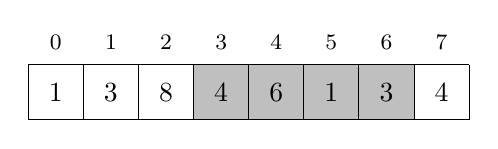
\begin{tikzpicture}[scale=0.7]
\fill[color=lightgray] (3,0) rectangle (7,1);
\draw (0,0) grid (8,1);

\node at (0.5,0.5) {$1$};
\node at (1.5,0.5) {$3$};
\node at (2.5,0.5) {$8$};
\node at (3.5,0.5) {$4$};
\node at (4.5,0.5) {$6$};
\node at (5.5,0.5) {$1$};
\node at (6.5,0.5) {$3$};
\node at (7.5,0.5) {$4$};

\footnotesize
\node at (0.5,1.4) {$0$};
\node at (1.5,1.4) {$1$};
\node at (2.5,1.4) {$2$};
\node at (3.5,1.4) {$3$};
\node at (4.5,1.4) {$4$};
\node at (5.5,1.4) {$5$};
\node at (6.5,1.4) {$6$};
\node at (7.5,1.4) {$7$};
\end{tikzpicture}
\end{center}
En este caso, $\texttt{sum}_q(3,6)=14$,
$\texttt{min}_q(3,6)=1$ y $\texttt{max}_q(3,6)=6$.

Una forma simple de procesar consultas de rango es usar
un bucle que recorra todos los valores de la matriz en el rango.
Por ejemplo, la siguiente función puede ser
usada para procesar consultas de suma en una matriz:

\begin{lstlisting}
int sum(int a, int b) {
    int s = 0;
    for (int i = a; i <= b; i++) {
        s += array[i];
    }
    return s;
}
\end{lstlisting}

Esta función funciona en tiempo $O(n)$,
donde $n$ es el tamaño de la matriz.
Por lo tanto, podemos procesar $q$ consultas en $O(nq)$
tiempo usando la función.
Sin embargo, si tanto $n$ como $q$ son grandes, este enfoque
es lento. Afortunadamente, resulta que hay
maneras de procesar consultas de rango mucho más eficientemente.

\section{Consultas de matriz estática}

Primero nos enfocamos en una situación donde
la matriz es \emph{estática}, es decir,
los valores de la matriz nunca se actualizan entre las consultas.
En este caso, es suficiente construir
una estructura de datos estática que nos diga
la respuesta para cualquier consulta posible.

\subsubsection{Consultas de suma}

\index{matriz de suma de prefijos}

Podemos procesar fácilmente
consultas de suma en una matriz estática
construyendo una \key{matriz de suma de prefijos}.
Cada valor en la matriz de suma de prefijos es igual
a la suma de los valores en la matriz original hasta esa posición,
es decir, el valor en la posición $k$ es $\texttt{sum}_q(0,k)$.
La matriz de suma de prefijos se puede construir en tiempo $O(n)$.

Por ejemplo, considere la siguiente matriz:
\begin{center}
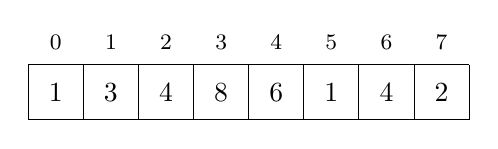
\begin{tikzpicture}[scale=0.7]
%\fill[color=lightgray] (3,0) rectangle (7,1);
\draw (0,0) grid (8,1);

\node at (0.5,0.5) {$1$};
\node at (1.5,0.5) {$3$};
\node at (2.5,0.5) {$4$};
\node at (3.5,0.5) {$8$};
\node at (4.5,0.5) {$6$};
\node at (5.5,0.5) {$1$};
\node at (6.5,0.5) {$4$};
\node at (7.5,0.5) {$2$};

\footnotesize
\node at (0.5,1.4) {$0$};
\node at (1.5,1.4) {$1$};
\node at (2.5,1.4) {$2$};
\node at (3.5,1.4) {$3$};
\node at (4.5,1.4) {$4$};
\node at (5.5,1.4) {$5$};
\node at (6.5,1.4) {$6$};
\node at (7.5,1.4) {$7$};
\end{tikzpicture}
\end{center}
La matriz de suma de prefijos correspondiente es la siguiente:
\begin{center}
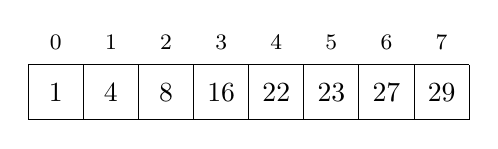
\begin{tikzpicture}[scale=0.7]
%\fill[color=lightgray] (3,0) rectangle (7,1);
\draw (0,0) grid (8,1);

\node at (0.5,0.5) {$1$};
\node at (1.5,0.5) {$4$};
\node at (2.5,0.5) {$8$};
\node at (3.5,0.5) {$16$};
\node at (4.5,0.5) {$22$};
\node at (5.5,0.5) {$23$};
\node at (6.5,0.5) {$27$};
\node at (7.5,0.5) {$29$};


\footnotesize
\node at (0.5,1.4) {$0$};
\node at (1.5,1.4) {$1$};
\node at (2.5,1.4) {$2$};
\node at (3.5,1.4) {$3$};
\node at (4.5,1.4) {$4$};
\node at (5.5,1.4) {$5$};
\node at (6.5,1.4) {$6$};
\node at (7.5,1.4) {$7$};
\end{tikzpicture}
\end{center}
Dado que la matriz de suma de prefijos contiene todos los valores
de $\texttt{sum}_q(0,k)$,
podemos calcular cualquier valor de
$\texttt{sum}_q(a,b)$ en tiempo $O(1)$ de la siguiente manera:
\[ \texttt{sum}_q(a,b) = \texttt{sum}_q(0,b) - \texttt{sum}_q(0,a-1)\]
Definiendo $\texttt{sum}_q(0,-1)=0$,
la fórmula anterior también se cumple cuando $a=0$.

Por ejemplo, considere el rango $[3,6]$:
\begin{center}
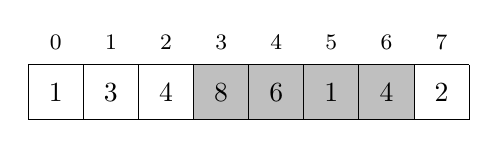
\begin{tikzpicture}[scale=0.7]
\fill[color=lightgray] (3,0) rectangle (7,1);
\draw (0,0) grid (8,1);

\node at (0.5,0.5) {$1$};
\node at (1.5,0.5) {$3$};
\node at (2.5,0.5) {$4$};
\node at (3.5,0.5) {$8$};
\node at (4.5,0.5) {$6$};
\node at (5.5,0.5) {$1$};
\node at (6.5,0.5) {$4$};
\node at (7.5,0.5) {$2$};



\footnotesize
\node at (0.5,1.4) {$0$};
\node at (1.5,1.4) {$1$};
\node at (2.5,1.4) {$2$};
\node at (3.5,1.4) {$3$};
\node at (4.5,1.4) {$4$};
\node at (5.5,1.4) {$5$};
\node at (6.5,1.4) {$6$};
\node at (7.5,1.4) {$7$};
\end{tikzpicture}
\end{center}
En este caso $\texttt{sum}_q(3,6)=8+6+1+4=19$.
Esta suma se puede calcular a partir de
dos valores del arreglo de suma de prefijo:
\begin{center}
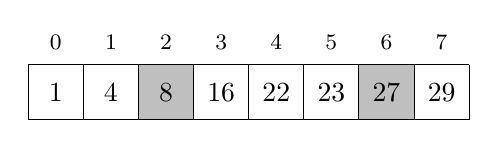
\begin{tikzpicture}[scale=0.7]
\fill[color=lightgray] (2,0) rectangle (3,1);
\fill[color=lightgray] (6,0) rectangle (7,1);
\draw (0,0) grid (8,1);

\node at (0.5,0.5) {$1$};
\node at (1.5,0.5) {$4$};
\node at (2.5,0.5) {$8$};
\node at (3.5,0.5) {$16$};
\node at (4.5,0.5) {$22$};
\node at (5.5,0.5) {$23$};
\node at (6.5,0.5) {$27$};
\node at (7.5,0.5) {$29$};

\footnotesize
\node at (0.5,1.4) {$0$};
\node at (1.5,1.4) {$1$};
\node at (2.5,1.4) {$2$};
\node at (3.5,1.4) {$3$};
\node at (4.5,1.4) {$4$};
\node at (5.5,1.4) {$5$};
\node at (6.5,1.4) {$6$};
\node at (7.5,1.4) {$7$};
\end{tikzpicture}
\end{center}
Por lo tanto, $\texttt{sum}_q(3,6)=\texttt{sum}_q(0,6)-\texttt{sum}_q(0,2)=27-8=19$.

También es posible generalizar esta idea
a dimensiones superiores.
Por ejemplo, podemos construir un arreglo de suma de prefijo bidimensional
que se puede usar para calcular
la suma de cualquier subarreglo rectangular en tiempo $O(1)$.
Cada suma en tal arreglo corresponde a
un subarreglo
que comienza en la esquina superior izquierda del arreglo.

\begin{samepage}
La siguiente imagen ilustra la idea:
\begin{center}
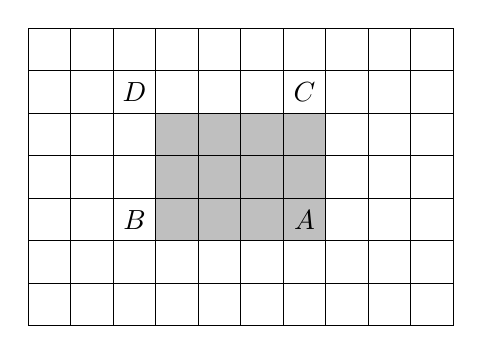
\begin{tikzpicture}[scale=0.54]
\draw[fill=lightgray] (3,2) rectangle (7,5);
\draw (0,0) grid (10,7);
\node[anchor=center] at (6.5, 2.5) {$A$};
\node[anchor=center] at (2.5, 2.5) {$B$};
\node[anchor=center] at (6.5, 5.5) {$C$};
\node[anchor=center] at (2.5, 5.5) {$D$};
\end{tikzpicture}
\end{center}
\end{samepage}

La suma del subarreglo gris se puede calcular
usando la fórmula
\[S(A) - S(B) - S(C) + S(D),\]
donde $S(X)$ denota la suma de valores
en un subarreglo rectangular
desde la esquina superior izquierda
hasta la posición de $X$.

\subsubsection{Consultas mínimas}

\index{tabla dispersa}

Las consultas mínimas son más difíciles de procesar
que las consultas de suma.
Aún así, existe un método de preprocesamiento bastante simple de
$O(n \log n)$ tiempo
después del cual podemos responder cualquier consulta mínima
en tiempo $O(1)$\footnote{Esta técnica
fue introducida en \cite{ben00} y a veces
se llama el método de la \key{tabla dispersa}.
También hay técnicas más sofisticadas \cite{fis06} donde
el tiempo de preprocesamiento es solo $O(n)$, pero tales algoritmos
no son necesarios en la programación competitiva.}.
Tenga en cuenta que dado que las consultas mínimas y máximas pueden
procesarse de forma similar,
podemos centrarnos en las consultas mínimas.

La idea es precalcular todos los valores de
$\textrm{min}_q(a,b)$ donde
$b-a+1$ (la longitud del rango) es una potencia de dos.
Por ejemplo, para el arreglo

\begin{center}
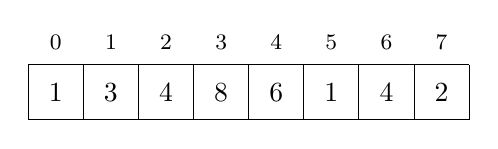
\begin{tikzpicture}[scale=0.7]
\draw (0,0) grid (8,1);

\node at (0.5,0.5) {$1$};
\node at (1.5,0.5) {$3$};
\node at (2.5,0.5) {$4$};
\node at (3.5,0.5) {$8$};
\node at (4.5,0.5) {$6$};
\node at (5.5,0.5) {$1$};
\node at (6.5,0.5) {$4$};
\node at (7.5,0.5) {$2$};

\footnotesize
\node at (0.5,1.4) {$0$};
\node at (1.5,1.4) {$1$};
\node at (2.5,1.4) {$2$};
\node at (3.5,1.4) {$3$};
\node at (4.5,1.4) {$4$};
\node at (5.5,1.4) {$5$};
\node at (6.5,1.4) {$6$};
\node at (7.5,1.4) {$7$};
\end{tikzpicture}
\end{center}
se calculan los siguientes valores:

\begin{center}
\begin{tabular}{ccc}

\begin{tabular}{lll}
$a$ & $b$ & $\texttt{min}_q(a,b)$ \\
\hline
0 & 0 & 1 \\
1 & 1 & 3 \\
2 & 2 & 4 \\
3 & 3 & 8 \\
4 & 4 & 6 \\
5 & 5 & 1 \\
6 & 6 & 4 \\
7 & 7 & 2 \\
\end{tabular}

&

\begin{tabular}{lll}
$a$ & $b$ & $\texttt{min}_q(a,b)$ \\
\hline
0 & 1 & 1 \\
1 & 2 & 3 \\
2 & 3 & 4 \\
3 & 4 & 6 \\
4 & 5 & 1 \\
5 & 6 & 1 \\
6 & 7 & 2 \\
\\
\end{tabular}

&

\begin{tabular}{lll}
$a$ & $b$ & $\texttt{min}_q(a,b)$ \\
\hline
0 & 3 & 1 \\
1 & 4 & 3 \\
2 & 5 & 1 \\
3 & 6 & 1 \\
4 & 7 & 1 \\
0 & 7 & 1 \\
\\
\\
\end{tabular}

\end{tabular}
\end{center}

El número de valores precalculados es $O(n \log n)$,
porque hay $O(\log n)$ longitudes de rango
que son potencias de dos.
Los valores se pueden calcular de manera eficiente
usando la fórmula recursiva
\[\texttt{min}_q(a,b) = \min(\texttt{min}_q(a,a+w-1),\texttt{min}_q(a+w,b)),\]
donde $b-a+1$ es una potencia de dos y $w=(b-a+1)/2$.
Calcular todos esos valores toma $O(n \log n)$ tiempo.

Después de esto, cualquier valor de $\texttt{min}_q(a,b)$ se puede calcular
en tiempo $O(1)$ como un mínimo de dos valores precalculados.
Sea $k$ la mayor potencia de dos que no excede $b-a+1$.
Podemos calcular el valor de $\texttt{min}_q(a,b)$ usando la fórmula
\[\texttt{min}_q(a,b) = \min(\texttt{min}_q(a,a+k-1),\texttt{min}_q(b-k+1,b)).\]
En la fórmula anterior, el rango $[a,b]$ está representado
como la unión de los rangos $[a,a+k-1]$ y $[b-k+1,b]$, ambos de longitud $k$.

Como ejemplo, considere el rango $[1,6]$:
\begin{center}
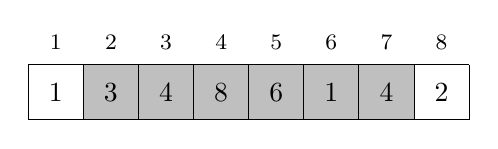
\begin{tikzpicture}[scale=0.7]
\fill[color=lightgray] (1,0) rectangle (7,1);
\draw (0,0) grid (8,1);

\node at (0.5,0.5) {$1$};
\node at (1.5,0.5) {$3$};
\node at (2.5,0.5) {$4$};
\node at (3.5,0.5) {$8$};
\node at (4.5,0.5) {$6$};
\node at (5.5,0.5) {$1$};
\node at (6.5,0.5) {$4$};
\node at (7.5,0.5) {$2$};

\footnotesize
\node at (0.5,1.4) {$1$};
\node at (1.5,1.4) {$2$};
\node at (2.5,1.4) {$3$};
\node at (3.5,1.4) {$4$};
\node at (4.5,1.4) {$5$};
\node at (5.5,1.4) {$6$};
\node at (6.5,1.4) {$7$};
\node at (7.5,1.4) {$8$};
\end{tikzpicture}
\end{center}
La longitud del rango es 6,
y la mayor potencia de dos que no
excede 6 es 4.
Por lo tanto, el rango $[1,6]$ es
la unión de los rangos $[1,4]$ y $[3,6]$:
\begin{center}
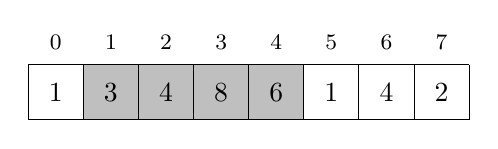
\begin{tikzpicture}[scale=0.7]
\fill[color=lightgray] (1,0) rectangle (5,1);
\draw (0,0) grid (8,1);

\node at (0.5,0.5) {$1$};
\node at (1.5,0.5) {$3$};
\node at (2.5,0.5) {$4$};
\node at (3.5,0.5) {$8$};
\node at (4.5,0.5) {$6$};
\node at (5.5,0.5) {$1$};
\node at (6.5,0.5) {$4$};
\node at (7.5,0.5) {$2$};

\footnotesize
\node at (0.5,1.4) {$0$};
\node at (1.5,1.4) {$1$};
\node at (2.5,1.4) {$2$};
\node at (3.5,1.4) {$3$};
\node at (4.5,1.4) {$4$};
\node at (5.5,1.4) {$5$};
\node at (6.5,1.4) {$6$};
\node at (7.5,1.4) {$7$};
\end{tikzpicture}
\end{center}
\begin{center}
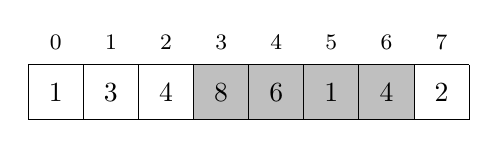
\begin{tikzpicture}[scale=0.7]
\fill[color=lightgray] (3,0) rectangle (7,1);
\draw (0,0) grid (8,1);

\node at (0.5,0.5) {$1$};
\node at (1.5,0.5) {$3$};
\node at (2.5,0.5) {$4$};
\node at (3.5,0.5) {$8$};
\node at (4.5,0.5) {$6$};
\node at (5.5,0.5) {$1$};
\node at (6.5,0.5) {$4$};
\node at (7.5,0.5) {$2$};


\footnotesize
\node at (0.5,1.4) {$0$};
\node at (1.5,1.4) {$1$};
\node at (2.5,1.4) {$2$};
\node at (3.5,1.4) {$3$};
\node at (4.5,1.4) {$4$};
\node at (5.5,1.4) {$5$};
\node at (6.5,1.4) {$6$};
\node at (7.5,1.4) {$7$};
\end{tikzpicture}
\end{center}
Dado que $\texttt{min}_q(1,4)=3$ y $\texttt{min}_q(3,6)=1$,
concluimos que $\texttt{min}_q(1,6)=1$.

\section{Árbol indexado binario}

\index{árbol indexado binario}
\index{árbol de Fenwick}

Un \key{árbol indexado binario} o un \key{árbol de Fenwick}\footnote{La
estructura del árbol indexado binario fue presentada por P. M. Fenwick en 1994 \cite{fen94}.}
se puede ver como una variante dinámica de una matriz de suma de prefijos.
Soporta dos operaciones en tiempo $O(\log n)$ en una matriz:
procesar una consulta de suma de rango y actualizar un valor.

La ventaja de un árbol indexado binario es
que nos permite actualizar de manera eficiente
los valores de la matriz entre consultas de suma.
Esto no sería posible usando una matriz de suma de prefijos,
porque después de cada actualización, sería necesario construir la
matriz de suma de prefijos completa nuevamente en tiempo $O(n)$.

\subsubsection{Estructura}

Incluso si el nombre de la estructura es un \emph{árbol} indexado binario,
generalmente se representa como una matriz.
En esta sección, asumimos que todas las matrices tienen índice uno,
porque facilita la implementación.

Sea $p(k)$ la mayor potencia de dos que
divide $k$.
Almacenamos un árbol indexado binario como una matriz \texttt{tree}
tal que
\[ \texttt{tree}[k] = \texttt{sum}_q(k-p(k)+1,k),\]
es decir, cada posición $k$ contiene la suma de los valores
en un rango de la matriz original cuya longitud es $p(k)$
y que termina en la posición $k$.
Por ejemplo, dado que $p(6)=2$, $\texttt{tree}[6]$
contiene el valor de $\texttt{sum}_q(5,6)$.

Por ejemplo, considere la siguiente matriz:
\begin{center}
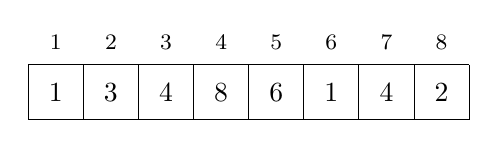
\begin{tikzpicture}[scale=0.7]
\draw (0,0) grid (8,1);

\node at (0.5,0.5) {$1$};
\node at (1.5,0.5) {$3$};
\node at (2.5,0.5) {$4$};
\node at (3.5,0.5) {$8$};
\node at (4.5,0.5) {$6$};
\node at (5.5,0.5) {$1$};
\node at (6.5,0.5) {$4$};
\node at (7.5,0.5) {$2$};

\footnotesize
\node at (0.5,1.4) {$1$};
\node at (1.5,1.4) {$2$};
\node at (2.5,1.4) {$3$};
\node at (3.5,1.4) {$4$};
\node at (4.5,1.4) {$5$};
\node at (5.5,1.4) {$6$};
\node at (6.5,1.4) {$7$};
\node at (7.5,1.4) {$8$};
\end{tikzpicture}
\end{center}

El árbol indexado binario correspondiente es el siguiente:
\begin{center}
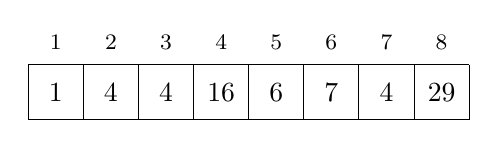
\begin{tikzpicture}[scale=0.7]
\draw (0,0) grid (8,1);

\node at (0.5,0.5) {$1$};
\node at (1.5,0.5) {$4$};
\node at (2.5,0.5) {$4$};
\node at (3.5,0.5) {$16$};
\node at (4.5,0.5) {$6$};
\node at (5.5,0.5) {$7$};
\node at (6.5,0.5) {$4$};
\node at (7.5,0.5) {$29$};

\footnotesize
\node at (0.5,1.4) {$1$};
\node at (1.5,1.4) {$2$};
\node at (2.5,1.4) {$3$};
\node at (3.5,1.4) {$4$};
\node at (4.5,1.4) {$5$};
\node at (5.5,1.4) {$6$};
\node at (6.5,1.4) {$7$};
\node at (7.5,1.4) {$8$};
\end{tikzpicture}
\end{center}

La siguiente imagen muestra más claramente
cómo cada valor en el árbol indexado binario
corresponde a un rango en la matriz original:

\begin{center}
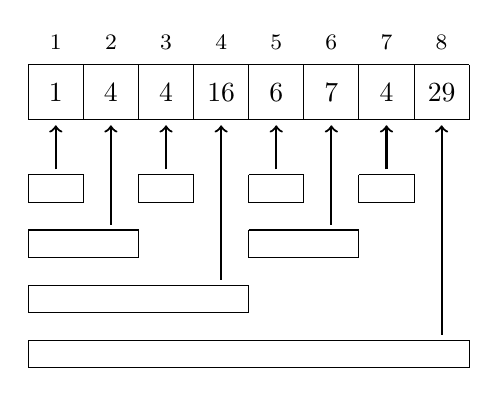
\begin{tikzpicture}[scale=0.7]
\draw (0,0) grid (8,1);

\node at (0.5,0.5) {$1$};
\node at (1.5,0.5) {$4$};
\node at (2.5,0.5) {$4$};
\node at (3.5,0.5) {$16$};
\node at (4.5,0.5) {$6$};
\node at (5.5,0.5) {$7$};
\node at (6.5,0.5) {$4$};
\node at (7.5,0.5) {$29$};

\footnotesize
\node at (0.5,1.4) {$1$};
\node at (1.5,1.4) {$2$};
\node at (2.5,1.4) {$3$};
\node at (3.5,1.4) {$4$};
\node at (4.5,1.4) {$5$};
\node at (5.5,1.4) {$6$};
\node at (6.5,1.4) {$7$};
\node at (7.5,1.4) {$8$};

\draw[->,thick] (0.5,-0.9) -- (0.5,-0.1);
\draw[->,thick] (2.5,-0.9) -- (2.5,-0.1);
\draw[->,thick] (4.5,-0.9) -- (4.5,-0.1);
\draw[->,thick] (6.5,-0.9) -- (6.5,-0.1);
\draw[->,thick] (1.5,-1.9) -- (1.5,-0.1);
\draw[->,thick] (5.5,-1.9) -- (5.5,-0.1);
\draw[->,thick] (3.5,-2.9) -- (3.5,-0.1);
\draw[->,thick] (7.5,-3.9) -- (7.5,-0.1);

\draw (0,-1) -- (1,-1) -- (1,-1.5) -- (0,-1.5) -- (0,-1);
\draw (2,-1) -- (3,-1) -- (3,-1.5) -- (2,-1.5) -- (2,-1);
\draw (4,-1) -- (5,-1) -- (5,-1.5) -- (4,-1.5) -- (4,-1);
\draw (6,-1) -- (7,-1) -- (7,-1.5) -- (6,-1.5) -- (6,-1);
\draw (0,-2) -- (2,-2) -- (2,-2.5) -- (0,-2.5) -- (0,-2);
\draw (4,-2) -- (6,-2) -- (6,-2.5) -- (4,-2.5) -- (4,-2);
\draw (0,-3) -- (4,-3) -- (4,-3.5) -- (0,-3.5) -- (0,-3);
\draw (0,-4) -- (8,-4) -- (8,-4.5) -- (0,-4.5) -- (0,-4);
\end{tikzpicture}
\end{center}

Usando un árbol indexado binario,
cualquier valor de $\texttt{sum}_q(1,k)$
se puede calcular en tiempo $O(\log n)$,
porque un rango $[1,k]$ siempre se puede dividir en
$O(\log n)$ rangos cuyas sumas están almacenadas en el árbol.

Por ejemplo, el rango $[1,7]$ consiste en
los siguientes rangos:
\begin{center}
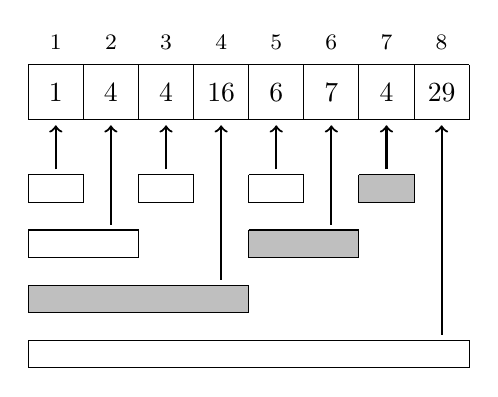
\begin{tikzpicture}[scale=0.7]
\draw (0,0) grid (8,1);

\node at (0.5,0.5) {$1$};
\node at (1.5,0.5) {$4$};
\node at (2.5,0.5) {$4$};
\node at (3.5,0.5) {$16$};
\node at (4.5,0.5) {$6$};
\node at (5.5,0.5) {$7$};
\node at (6.5,0.5) {$4$};
\node at (7.5,0.5) {$29$};

\footnotesize
\node at (0.5,1.4) {$1$};
\node at (1.5,1.4) {$2$};
\node at (2.5,1.4) {$3$};
\node at (3.5,1.4) {$4$};
\node at (4.5,1.4) {$5$};
\node at (5.5,1.4) {$6$};
\node at (6.5,1.4) {$7$};
\node at (7.5,1.4) {$8$};

\draw[->,thick] (0.5,-0.9) -- (0.5,-0.1);
\draw[->,thick] (2.5,-0.9) -- (2.5,-0.1);
\draw[->,thick] (4.5,-0.9) -- (4.5,-0.1);
\draw[->,thick] (6.5,-0.9) -- (6.5,-0.1);
\draw[->,thick] (1.5,-1.9) -- (1.5,-0.1);
\draw[->,thick] (5.5,-1.9) -- (5.5,-0.1);
\draw[->,thick] (3.5,-2.9) -- (3.5,-0.1);
\draw[->,thick] (7.5,-3.9) -- (7.5,-0.1);

\draw (0,-1) -- (1,-1) -- (1,-1.5) -- (0,-1.5) -- (0,-1);
\draw (2,-1) -- (3,-1) -- (3,-1.5) -- (2,-1.5) -- (2,-1);
\draw (4,-1) -- (5,-1) -- (5,-1.5) -- (4,-1.5) -- (4,-1);
\draw[fill=lightgray] (6,-1) -- (7,-1) -- (7,-1.5) -- (6,-1.5) -- (6,-1);
\draw (0,-2) -- (2,-2) -- (2,-2.5) -- (0,-2.5) -- (0,-2);
\draw[fill=lightgray] (4,-2) -- (6,-2) -- (6,-2.5) -- (4,-2.5) -- (4,-2);
\draw[fill=lightgray] (0,-3) -- (4,-3) -- (4,-3.5) -- (0,-3.5) -- (0,-3);
\draw (0,-4) -- (8,-4) -- (8,-4.5) -- (0,-4.5) -- (0,-4);
\end{tikzpicture}
\end{center}
Por lo tanto, podemos calcular la suma correspondiente de la siguiente manera:
\[\texttt{sum}_q(1,7)=\texttt{sum}_q(1,4)+\texttt{sum}_q(5,6)+\texttt{sum}_q(7,7)=16+7+4=27\]

Para calcular el valor de $\texttt{sum}_q(a,b)$ donde $a>1$,
podemos usar el mismo truco que usamos con las matrices de suma de prefijo:
\[ \texttt{sum}_q(a,b) = \texttt{sum}_q(1,b) - \texttt{sum}_q(1,a-1).\]
Dado que podemos calcular tanto $\texttt{sum}_q(1,b)$
como $\texttt{sum}_q(1,a-1)$ en tiempo $O(\log n)$,
la complejidad de tiempo total es $O(\log n)$.

Entonces, después de actualizar un valor en la matriz original,
varios valores en el árbol indexado binario
deberían actualizarse.
Por ejemplo, si el valor en la posición 3 cambia,
las sumas de los siguientes rangos cambian:
\begin{center}
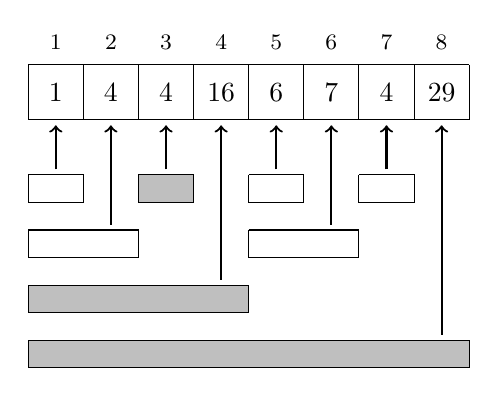
\begin{tikzpicture}[scale=0.7]
\draw (0,0) grid (8,1);

\node at (0.5,0.5) {$1$};
\node at (1.5,0.5) {$4$};
\node at (2.5,0.5) {$4$};
\node at (3.5,0.5) {$16$};
\node at (4.5,0.5) {$6$};
\node at (5.5,0.5) {$7$};
\node at (6.5,0.5) {$4$};
\node at (7.5,0.5) {$29$};

\footnotesize
\node at (0.5,1.4) {$1$};
\node at (1.5,1.4) {$2$};
\node at (2.5,1.4) {$3$};
\node at (3.5,1.4) {$4$};
\node at (4.5,1.4) {$5$};
\node at (5.5,1.4) {$6$};
\node at (6.5,1.4) {$7$};
\node at (7.5,1.4) {$8$};

\draw[->,thick] (0.5,-0.9) -- (0.5,-0.1);
\draw[->,thick] (2.5,-0.9) -- (2.5,-0.1);
\draw[->,thick] (4.5,-0.9) -- (4.5,-0.1);
\draw[->,thick] (6.5,-0.9) -- (6.5,-0.1);
\draw[->,thick] (1.5,-1.9) -- (1.5,-0.1);
\draw[->,thick] (5.5,-1.9) -- (5.5,-0.1);
\draw[->,thick] (3.5,-2.9) -- (3.5,-0.1);
\draw[->,thick] (7.5,-3.9) -- (7.5,-0.1);

\draw (0,-1) -- (1,-1) -- (1,-1.5) -- (0,-1.5) -- (0,-1);
\draw[fill=lightgray] (2,-1) -- (3,-1) -- (3,-1.5) -- (2,-1.5) -- (2,-1);
\draw (4,-1) -- (5,-1) -- (5,-1.5) -- (4,-1.5) -- (4,-1);
\draw (6,-1) -- (7,-1) -- (7,-1.5) -- (6,-1.5) -- (6,-1);
\draw (0,-2) -- (2,-2) -- (2,-2.5) -- (0,-2.5) -- (0,-2);
\draw (4,-2) -- (6,-2) -- (6,-2.5) -- (4,-2.5) -- (4,-2);
\draw[fill=lightgray] (0,-3) -- (4,-3) -- (4,-3.5) -- (0,-3.5) -- (0,-3);
\draw[fill=lightgray] (0,-4) -- (8,-4) -- (8,-4.5) -- (0,-4.5) -- (0,-4);
\end{tikzpicture}
\end{center}

Dado que cada elemento de la matriz pertenece a $O(\log n)$
rangos en el árbol indexado binario,
es suficiente actualizar $O(\log n)$ valores en el árbol.

\subsubsection{Implementación}


Las operaciones de un árbol indexado binario se pueden
implementar eficientemente utilizando operaciones de bits.
El hecho clave que se necesita es que podemos
calcular cualquier valor de $p(k)$ utilizando la fórmula
\[p(k) = k \& -k.\]

La siguiente función calcula el valor de $\texttt{sum}_q(1,k)$:
\begin{lstlisting}
int sum(int k) {
    int s = 0;
    while (k >= 1) {
        s += tree[k];
        k -= k&-k;
    }
    return s;
}
\end{lstlisting}

La siguiente función incrementa el
valor del arreglo en la posición $k$ por $x$
($x$ puede ser positivo o negativo):
\begin{lstlisting}
void add(int k, int x) {
    while (k <= n) {
        tree[k] += x;
        k += k&-k;
    }
}
\end{lstlisting}

La complejidad temporal de ambas funciones es
$O(\log n)$, porque las funciones acceden a $O(\log n)$
valores en el árbol indexado binario, y cada movimiento
a la siguiente posición toma $O(1)$ tiempo.

\section{Árbol de segmentos}

\index{árbol de segmentos}

Un \key{árbol de segmentos}\footnote{La implementación ascendente en este capítulo corresponde a
la de \cite{sta06}. Estructuras similares se usaron
a finales de la década de 1970 para resolver problemas geométricos \cite{ben80}.} es una estructura de datos
que admite dos operaciones:
procesamiento de una consulta de rango y
actualización de un valor del arreglo.
Los árboles de segmentos pueden admitir
consultas de suma, consultas de mínimo y máximo y muchas otras
consultas para que ambas operaciones funcionen en $O(\log n)$ tiempo.

En comparación con un árbol indexado binario,
la ventaja de un árbol de segmentos es que es
una estructura de datos más general.
Mientras que los árboles indexados binarios solo admiten
consultas de suma\footnote{De hecho, utilizando \emph{dos} árboles indexados binarios es posible admitir consultas de mínimo \cite{dim15},
pero esto es más complicado que usar un árbol de segmentos.},
los árboles de segmentos también admiten otras consultas.
Por otro lado, un árbol de segmentos requiere más
memoria y es un poco más difícil de implementar.

\subsubsection{Estructura}

Un árbol de segmentos es un árbol binario
tal que los nodos en el nivel inferior del árbol
corresponden a los elementos del arreglo,
y los otros nodos
contienen información necesaria para procesar consultas de rango.

En esta sección, asumimos que el tamaño
del arreglo es una potencia de dos y se utiliza un índice basado en cero, porque es conveniente construir
un árbol de segmentos para tal arreglo.
Si el tamaño del arreglo no es una potencia de dos,
siempre podemos agregar elementos adicionales a él.

Primero discutiremos los árboles de segmentos que admiten consultas de suma.
Como ejemplo, considere el siguiente arreglo:
\begin{center}
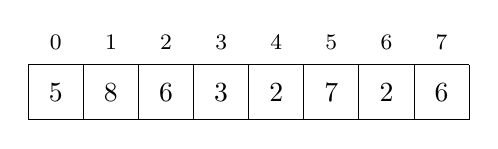
\begin{tikzpicture}[scale=0.7]
\draw (0,0) grid (8,1);

\node at (0.5,0.5) {$5$};
\node at (1.5,0.5) {$8$};
\node at (2.5,0.5) {$6$};
\node at (3.5,0.5) {$3$};
\node at (4.5,0.5) {$2$};
\node at (5.5,0.5) {$7$};
\node at (6.5,0.5) {$2$};
\node at (7.5,0.5) {$6$};

\footnotesize
\node at (0.5,1.4) {$0$};
\node at (1.5,1.4) {$1$};
\node at (2.5,1.4) {$2$};
\node at (3.5,1.4) {$3$};
\node at (4.5,1.4) {$4$};
\node at (5.5,1.4) {$5$};
\node at (6.5,1.4) {$6$};
\node at (7.5,1.4) {$7$};
\end{tikzpicture}
\end{center}
El árbol de segmentos correspondiente es el siguiente:
\begin{center}
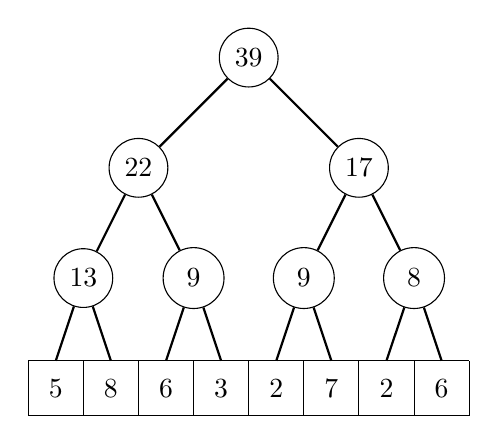
\begin{tikzpicture}[scale=0.7]
\draw (0,0) grid (8,1);

\node[anchor=center] at (0.5, 0.5) {5};
\node[anchor=center] at (1.5, 0.5) {8};
\node[anchor=center] at (2.5, 0.5) {6};
\node[anchor=center] at (3.5, 0.5) {3};
\node[anchor=center] at (4.5, 0.5) {2};
\node[anchor=center] at (5.5, 0.5) {7};
\node[anchor=center] at (6.5, 0.5) {2};
\node[anchor=center] at (7.5, 0.5) {6};

\node[draw, circle] (a) at (1,2.5) {13};
\path[draw,thick,-] (a) -- (0.5,1);
\path[draw,thick,-] (a) -- (1.5,1);
\node[draw, circle,minimum size=22pt] (b) at (3,2.5) {9};
\path[draw,thick,-] (b) -- (2.5,1);
\path[draw,thick,-] (b) -- (3.5,1);
\node[draw, circle,minimum size=22pt] (c) at (5,2.5) {9};
\path[draw,thick,-] (c) -- (4.5,1);
\path[draw,thick,-] (c) -- (5.5,1);
\node[draw, circle,minimum size=22pt] (d) at (7,2.5) {8};
\path[draw,thick,-] (d) -- (6.5,1);
\path[draw,thick,-] (d) -- (7.5,1);

\node[draw, circle] (i) at (2,4.5) {22};
\path[draw,thick,-] (i) -- (a);
\path[draw,thick,-] (i) -- (b);
\node[draw, circle] (j) at (6,4.5) {17};
\path[draw,thick,-] (j) -- (c);
\path[draw,thick,-] (j) -- (d);

\node[draw, circle] (m) at (4,6.5) {39};
\path[draw,thick,-] (m) -- (i);
\path[draw,thick,-] (m) -- (j);
\end{tikzpicture}
\end{center}

Cada nodo interno del árbol
corresponde a un rango del arreglo
cuyo tamaño es una potencia de dos.
En el árbol anterior, el valor de cada interno
nodo es la suma de los valores del arreglo correspondientes,
y se puede calcular como la suma de
los valores de su nodo hijo izquierdo y derecho.

Resulta que cualquier rango $[a,b]$
se puede dividir en $O(\log n)$ rangos
cuyos valores se almacenan en nodos del árbol.
Por ejemplo, considere el rango [2,7]:
\begin{center}
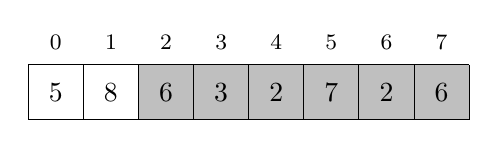
\begin{tikzpicture}[scale=0.7]
\fill[color=gray!50] (2,0) rectangle (8,1);
\draw (0,0) grid (8,1);
\node[anchor=center] at (0.5, 0.5) {5};
\node[anchor=center] at (1.5, 0.5) {8};
\node[anchor=center] at (2.5, 0.5) {6};
\node[anchor=center] at (3.5, 0.5) {3};
\node[anchor=center] at (4.5, 0.5) {2};
\node[anchor=center] at (5.5, 0.5) {7};
\node[anchor=center] at (6.5, 0.5) {2};
\node[anchor=center] at (7.5, 0.5) {6};

\footnotesize
\node at (0.5,1.4) {$0$};
\node at (1.5,1.4) {$1$};
\node at (2.5,1.4) {$2$};
\node at (3.5,1.4) {$3$};
\node at (4.5,1.4) {$4$};
\node at (5.5,1.4) {$5$};
\node at (6.5,1.4) {$6$};
\node at (7.5,1.4) {$7$};
\end{tikzpicture}
\end{center}
Aquí $\texttt{sum}_q(2,7)=6+3+2+7+2+6=26$.
En este caso, los dos siguientes nodos del árbol
corresponden al rango:
\begin{center}
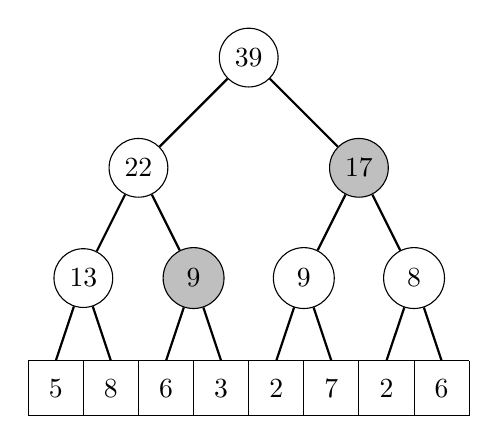
\begin{tikzpicture}[scale=0.7]
\draw (0,0) grid (8,1);

\node[anchor=center] at (0.5, 0.5) {5};
\node[anchor=center] at (1.5, 0.5) {8};
\node[anchor=center] at (2.5, 0.5) {6};
\node[anchor=center] at (3.5, 0.5) {3};
\node[anchor=center] at (4.5, 0.5) {2};
\node[anchor=center] at (5.5, 0.5) {7};
\node[anchor=center] at (6.5, 0.5) {2};
\node[anchor=center] at (7.5, 0.5) {6};

\node[draw, circle] (a) at (1,2.5) {13};
\path[draw,thick,-] (a) -- (0.5,1);
\path[draw,thick,-] (a) -- (1.5,1);
\node[draw, circle,fill=gray!50,minimum size=22pt] (b) at (3,2.5) {9};
\path[draw,thick,-] (b) -- (2.5,1);
\path[draw,thick,-] (b) -- (3.5,1);
\node[draw, circle,minimum size=22pt] (c) at (5,2.5) {9};
\path[draw,thick,-] (c) -- (4.5,1);
\path[draw,thick,-] (c) -- (5.5,1);
\node[draw, circle,minimum size=22pt] (d) at (7,2.5) {8};
\path[draw,thick,-] (d) -- (6.5,1);
\path[draw,thick,-] (d) -- (7.5,1);

\node[draw, circle] (i) at (2,4.5) {22};
\path[draw,thick,-] (i) -- (a);
\path[draw,thick,-] (i) -- (b);
\node[draw, circle,fill=gray!50] (j) at (6,4.5) {17};
\path[draw,thick,-] (j) -- (c);
\path[draw,thick,-] (j) -- (d);

\node[draw, circle] (m) at (4,6.5) {39};
\path[draw,thick,-] (m) -- (i);
\path[draw,thick,-] (m) -- (j);
\end{tikzpicture}
\end{center}
Por lo tanto, otra forma de calcular la suma es $9+17=26$.

Cuando la suma se calcula usando nodos
ubicados lo más alto posible en el árbol,
como máximo dos nodos en cada nivel
del árbol son necesarios.
Por lo tanto, el número total de nodos
es $O(\log n)$.

Después de una actualización de la matriz,
deberíamos actualizar todos los nodos
cuyo valor depende del valor actualizado.
Esto se puede hacer recorriendo la ruta
desde el elemento de la matriz actualizado hasta el nodo superior
y actualizando los nodos a lo largo de la ruta.

La siguiente imagen muestra qué nodos del árbol
cambian si el valor de la matriz 7 cambia:

\begin{center}
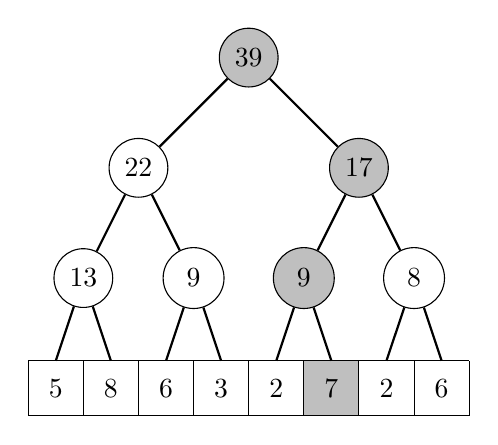
\begin{tikzpicture}[scale=0.7]
\fill[color=gray!50] (5,0) rectangle (6,1);
\draw (0,0) grid (8,1);

\node[anchor=center] at (0.5, 0.5) {5};
\node[anchor=center] at (1.5, 0.5) {8};
\node[anchor=center] at (2.5, 0.5) {6};
\node[anchor=center] at (3.5, 0.5) {3};
\node[anchor=center] at (4.5, 0.5) {2};
\node[anchor=center] at (5.5, 0.5) {7};
\node[anchor=center] at (6.5, 0.5) {2};
\node[anchor=center] at (7.5, 0.5) {6};

\node[draw, circle] (a) at (1,2.5) {13};
\path[draw,thick,-] (a) -- (0.5,1);
\path[draw,thick,-] (a) -- (1.5,1);
\node[draw, circle,minimum size=22pt] (b) at (3,2.5) {9};
\path[draw,thick,-] (b) -- (2.5,1);
\path[draw,thick,-] (b) -- (3.5,1);
\node[draw, circle,minimum size=22pt,fill=gray!50] (c) at (5,2.5) {9};
\path[draw,thick,-] (c) -- (4.5,1);
\path[draw,thick,-] (c) -- (5.5,1);
\node[draw, circle,minimum size=22pt] (d) at (7,2.5) {8};
\path[draw,thick,-] (d) -- (6.5,1);
\path[draw,thick,-] (d) -- (7.5,1);

\node[draw, circle] (i) at (2,4.5) {22};
\path[draw,thick,-] (i) -- (a);
\path[draw,thick,-] (i) -- (b);
\node[draw, circle,fill=gray!50] (j) at (6,4.5) {17};
\path[draw,thick,-] (j) -- (c);
\path[draw,thick,-] (j) -- (d);

\node[draw, circle,fill=gray!50] (m) at (4,6.5) {39};
\path[draw,thick,-] (m) -- (i);
\path[draw,thick,-] (m) -- (j);
\end{tikzpicture}
\end{center}

La ruta de abajo hacia arriba
siempre consiste en $O(\log n)$ nodos,
por lo que cada actualización cambia $O(\log n)$ nodos en el árbol.

\subsubsection{Implementación}

Almacenamos un árbol de segmentos como una matriz
de $2n$ elementos donde $n$ es el tamaño de
la matriz original y una potencia de dos.
Los nodos del árbol se almacenan de arriba hacia abajo:
$\texttt{tree}[1]$ es el nodo superior,
$\texttt{tree}[2]$ y $\texttt{tree}[3]$
son sus hijos, y así sucesivamente.
Finalmente, los valores de $\texttt{tree}[n]$
a $\texttt{tree}[2n-1]$ corresponden a
los valores de la matriz original
en el nivel inferior del árbol.

Por ejemplo, el árbol de segmentos
\begin{center}
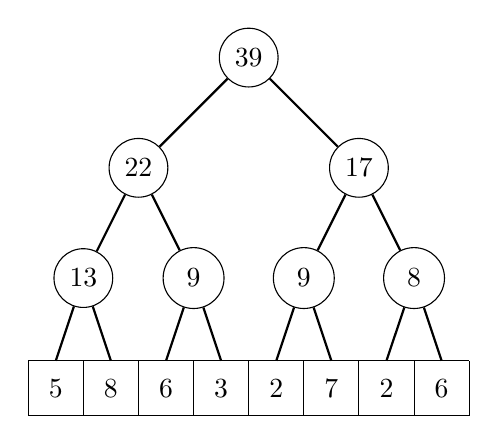
\begin{tikzpicture}[scale=0.7]
\draw (0,0) grid (8,1);

\node[anchor=center] at (0.5, 0.5) {5};
\node[anchor=center] at (1.5, 0.5) {8};
\node[anchor=center] at (2.5, 0.5) {6};
\node[anchor=center] at (3.5, 0.5) {3};
\node[anchor=center] at (4.5, 0.5) {2};
\node[anchor=center] at (5.5, 0.5) {7};
\node[anchor=center] at (6.5, 0.5) {2};
\node[anchor=center] at (7.5, 0.5) {6};

\node[draw, circle] (a) at (1,2.5) {13};
\path[draw,thick,-] (a) -- (0.5,1);
\path[draw,thick,-] (a) -- (1.5,1);
\node[draw, circle,minimum size=22pt] (b) at (3,2.5) {9};
\path[draw,thick,-] (b) -- (2.5,1);
\path[draw,thick,-] (b) -- (3.5,1);
\node[draw, circle,minimum size=22pt] (c) at (5,2.5) {9};
\path[draw,thick,-] (c) -- (4.5,1);
\path[draw,thick,-] (c) -- (5.5,1);
\node[draw, circle,minimum size=22pt] (d) at (7,2.5) {8};
\path[draw,thick,-] (d) -- (6.5,1);
\path[draw,thick,-] (d) -- (7.5,1);

\node[draw, circle] (i) at (2,4.5) {22};
\path[draw,thick,-] (i) -- (a);
\path[draw,thick,-] (i) -- (b);
\node[draw, circle] (j) at (6,4.5) {17};
\path[draw,thick,-] (j) -- (c);
\path[draw,thick,-] (j) -- (d);

\node[draw, circle] (m) at (4,6.5) {39};
\path[draw,thick,-] (m) -- (i);
\path[draw,thick,-] (m) -- (j);
\end{tikzpicture}
\end{center}
se almacena de la siguiente manera:
\begin{center}
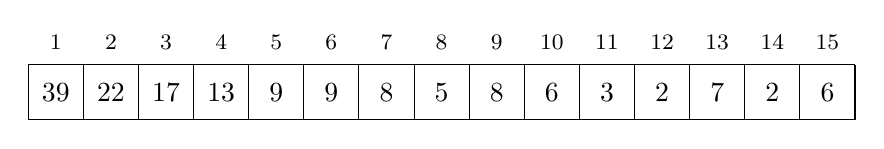
\begin{tikzpicture}[scale=0.7]
\draw (0,0) grid (15,1);

\node at (0.5,0.5) {$39$};
\node at (1.5,0.5) {$22$};
\node at (2.5,0.5) {$17$};
\node at (3.5,0.5) {$13$};
\node at (4.5,0.5) {$9$};
\node at (5.5,0.5) {$9$};
\node at (6.5,0.5) {$8$};
\node at (7.5,0.5) {$5$};
\node at (8.5,0.5) {$8$};
\node at (9.5,0.5) {$6$};
\node at (10.5,0.5) {$3$};
\node at (11.5,0.5) {$2$};
\node at (12.5,0.5) {$7$};
\node at (13.5,0.5) {$2$};
\node at (14.5,0.5) {$6$};

\footnotesize
\node at (0.5,1.4) {$1$};
\node at (1.5,1.4) {$2$};
\node at (2.5,1.4) {$3$};
\node at (3.5,1.4) {$4$};
\node at (4.5,1.4) {$5$};
\node at (5.5,1.4) {$6$};
\node at (6.5,1.4) {$7$};
\node at (7.5,1.4) {$8$};
\node at (8.5,1.4) {$9$};
\node at (9.5,1.4) {$10$};
\node at (10.5,1.4) {$11$};
\node at (11.5,1.4) {$12$};
\node at (12.5,1.4) {$13$};
\node at (13.5,1.4) {$14$};
\node at (14.5,1.4) {$15$};
\end{tikzpicture}
\end{center}
Usando esta representación,
el padre de $\texttt{tree}[k]$
es $\texttt{tree}[\lfloor k/2 \rfloor]$,
y sus hijos son $\texttt{tree}[2k]$
y $\texttt{tree}[2k+1]$.
Tenga en cuenta que esto implica que la posición de un nodo
es par si es un hijo izquierdo e impar si es un hijo derecho.

La siguiente función
calcula el valor de $\texttt{sum}_q(a,b)$:
\begin{lstlisting}
int sum(int a, int b) {
    a += n; b += n;
    int s = 0;
    while (a <= b) {
        if (a%2 == 1) s += tree[a++];
        if (b%2 == 0) s += tree[b--];
        a /= 2; b /= 2;
    }
    return s;
}
\end{lstlisting}
La función mantiene un rango
que es inicialmente $[a+n,b+n]$.
Luego, en cada paso, el rango se mueve
un nivel más alto en el árbol,
y antes de eso, los valores de los nodos que no
pertenecen al rango superior se agregan a la suma.

La siguiente función aumenta el valor de la matriz
en la posición $k$ en $x$:
\begin{lstlisting}
void add(int k, int x) {
    k += n;
    tree[k] += x;
    for (k /= 2; k >= 1; k /= 2) {
        tree[k] = tree[2*k]+tree[2*k+1];
    }
}
\end{lstlisting}
Primero, la función actualiza el valor
en el nivel inferior del árbol.
Después de esto, la función actualiza los valores de todos
los nodos internos del árbol, hasta que llega
al nodo superior del árbol.

Ambas funciones anteriores funcionan
en $O(\log n)$ tiempo, porque un árbol de segmentos
de $n$ elementos consta de $O(\log n)$ niveles,
y las funciones se mueven un nivel más alto
en el árbol en cada paso.

\subsubsection{Otras consultas}

Los árboles de segmentos pueden admitir todas las consultas de rango
donde es posible dividir un rango en dos partes,
calcular la respuesta por separado para ambas partes
y luego combinar las respuestas de manera eficiente.
Ejemplos de tales consultas son
mínimo y máximo, máximo común divisor,
y operaciones bit a bit y, o y xor.

Por ejemplo, el siguiente árbol de segmentos
admite consultas mínimas:

\begin{center}
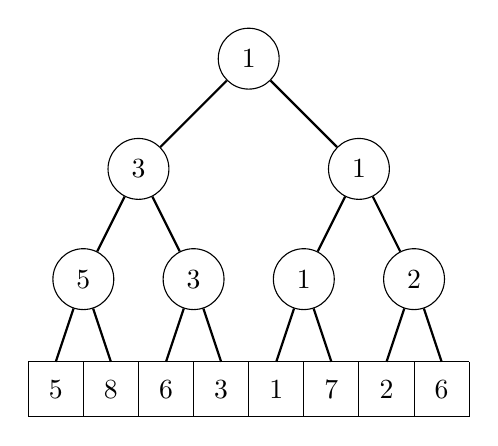
\begin{tikzpicture}[scale=0.7]
\draw (0,0) grid (8,1);

\node[anchor=center] at (0.5, 0.5) {5};
\node[anchor=center] at (1.5, 0.5) {8};
\node[anchor=center] at (2.5, 0.5) {6};
\node[anchor=center] at (3.5, 0.5) {3};
\node[anchor=center] at (4.5, 0.5) {1};
\node[anchor=center] at (5.5, 0.5) {7};
\node[anchor=center] at (6.5, 0.5) {2};
\node[anchor=center] at (7.5, 0.5) {6};

\node[draw, circle,minimum size=22pt] (a) at (1,2.5) {5};
\path[draw,thick,-] (a) -- (0.5,1);
\path[draw,thick,-] (a) -- (1.5,1);
\node[draw, circle,minimum size=22pt] (b) at (3,2.5) {3};
\path[draw,thick,-] (b) -- (2.5,1);
\path[draw,thick,-] (b) -- (3.5,1);
\node[draw, circle,minimum size=22pt] (c) at (5,2.5) {1};
\path[draw,thick,-] (c) -- (4.5,1);
\path[draw,thick,-] (c) -- (5.5,1);
\node[draw, circle,minimum size=22pt] (d) at (7,2.5) {2};
\path[draw,thick,-] (d) -- (6.5,1);
\path[draw,thick,-] (d) -- (7.5,1);

\node[draw, circle,minimum size=22pt] (i) at (2,4.5) {3};
\path[draw,thick,-] (i) -- (a);
\path[draw,thick,-] (i) -- (b);
\node[draw, circle,minimum size=22pt] (j) at (6,4.5) {1};
\path[draw,thick,-] (j) -- (c);
\path[draw,thick,-] (j) -- (d);

\node[draw, circle,minimum size=22pt] (m) at (4,6.5) {1};
\path[draw,thick,-] (m) -- (i);
\path[draw,thick,-] (m) -- (j);
\end{tikzpicture}
\end{center}
En este caso, cada nodo de árbol contiene
el valor más pequeño en el correspondiente
rango de la matriz.
El nodo superior del árbol contiene el más pequeño
valor en toda la matriz.
Las operaciones se pueden implementar como anteriormente,
pero en lugar de sumas, se calculan los mínimos.

La estructura de un árbol de segmentos también nos permite
usar la búsqueda binaria para localizar elementos de la matriz.
Por ejemplo, si el árbol admite consultas mínimas,
podemos encontrar la posición de un elemento
con el valor más pequeño en $O(\log n)$ tiempo.

Por ejemplo, en el árbol anterior, un
elemento con el valor más pequeño 1 se puede encontrar
atravesando un camino hacia abajo desde el nodo superior:

\begin{center}
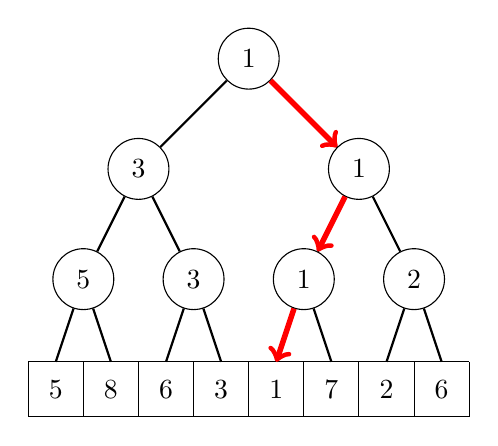
\begin{tikzpicture}[scale=0.7]
\draw (0,0) grid (8,1);

\node[anchor=center] at (0.5, 0.5) {5};
\node[anchor=center] at (1.5, 0.5) {8};
\node[anchor=center] at (2.5, 0.5) {6};
\node[anchor=center] at (3.5, 0.5) {3};
\node[anchor=center] at (4.5, 0.5) {1};
\node[anchor=center] at (5.5, 0.5) {7};
\node[anchor=center] at (6.5, 0.5) {2};
\node[anchor=center] at (7.5, 0.5) {6};

\node[draw, circle,minimum size=22pt] (a) at (1,2.5) {5};
\path[draw,thick,-] (a) -- (0.5,1);
\path[draw,thick,-] (a) -- (1.5,1);
\node[draw, circle,minimum size=22pt] (b) at (3,2.5) {3};
\path[draw,thick,-] (b) -- (2.5,1);
\path[draw,thick,-] (b) -- (3.5,1);
\node[draw, circle,minimum size=22pt] (c) at (5,2.5) {1};
\path[draw,thick,-] (c) -- (4.5,1);
\path[draw,thick,-] (c) -- (5.5,1);
\node[draw, circle,minimum size=22pt] (d) at (7,2.5) {2};
\path[draw,thick,-] (d) -- (6.5,1);
\path[draw,thick,-] (d) -- (7.5,1);

\node[draw, circle,minimum size=22pt] (i) at (2,4.5) {3};
\path[draw,thick,-] (i) -- (a);
\path[draw,thick,-] (i) -- (b);
\node[draw, circle,minimum size=22pt] (j) at (6,4.5) {1};
\path[draw,thick,-] (j) -- (c);
\path[draw,thick,-] (j) -- (d);

\node[draw, circle,minimum size=22pt] (m) at (4,6.5) {1};
\path[draw,thick,-] (m) -- (i);
\path[draw,thick,-] (m) -- (j);

\path[draw=red,thick,->,line width=2pt] (m) -- (j);
\path[draw=red,thick,->,line width=2pt] (j) -- (c);
\path[draw=red,thick,->,line width=2pt] (c) -- (4.5,1);
\end{tikzpicture}
\end{center}

\section{Técnicas adicionales}

\subsubsection{Compresión de índice}

Una limitación en las estructuras de datos que
se basan en una matriz es que
los elementos están indexados usando
enteros consecutivos.
Surgen dificultades cuando se necesitan índices grandes.
Por ejemplo, si queremos usar el índice $10^9$,
la matriz debe contener $10^9$
elementos que requerirían demasiada memoria.

\index{index compression}

Sin embargo, a menudo podemos evitar esta limitación
usando \key{compresión de índice},
donde los índices originales son reemplazados
por índices $1,2,3,$ etc.
Esto se puede hacer si conocemos todos los índices
necesitados durante el algoritmo de antemano.

La idea es reemplazar cada índice original $x$
con $c(x)$ donde $c$ es una función que
comprime los índices.
Requerimos que el orden de los índices
no cambie, así que si $a<b$, entonces $c(a)<c(b)$.
Esto nos permite realizar consultas convenientemente
incluso si los índices están comprimidos.

Por ejemplo, si los índices originales son
$555$, $10^9$ y $8$, los nuevos índices son:

\[
\begin{array}{lcl}
c(8) & = & 1 \\
c(555) & = & 2 \\
c(10^9) & = & 3 \\
\end{array}
\]

\subsubsection{Actualizaciones de rango}

Hasta ahora, hemos implementado estructuras de datos
que admiten consultas de rango y actualizaciones
de valores únicos.
Consideremos ahora una situación opuesta,
donde deberíamos actualizar rangos y
recuperar valores únicos.
Nos enfocamos en una operación que aumenta todos
los elementos en un rango $[a,b]$ por $x$.

\index{difference array}

Sorprendentemente, podemos usar las estructuras de datos
presentadas en este capítulo también en esta situación.
Para hacer esto, construimos una \key{matriz de diferencias}
cuyos valores indican
las diferencias entre valores consecutivos
en la matriz original.
Por lo tanto, la matriz original es la
matriz de suma de prefijo de la
matriz de diferencias.
Por ejemplo, considere la siguiente matriz:

\begin{center}
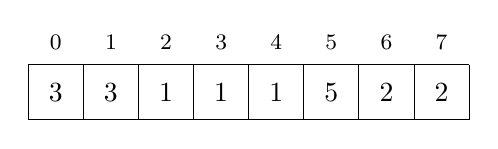
\begin{tikzpicture}[scale=0.7]
\draw (0,0) grid (8,1);

\node at (0.5,0.5) {$3$};
\node at (1.5,0.5) {$3$};
\node at (2.5,0.5) {$1$};
\node at (3.5,0.5) {$1$};
\node at (4.5,0.5) {$1$};
\node at (5.5,0.5) {$5$};
\node at (6.5,0.5) {$2$};
\node at (7.5,0.5) {$2$};


\footnotesize
\node at (0.5,1.4) {$0$};
\node at (1.5,1.4) {$1$};
\node at (2.5,1.4) {$2$};
\node at (3.5,1.4) {$3$};
\node at (4.5,1.4) {$4$};
\node at (5.5,1.4) {$5$};
\node at (6.5,1.4) {$6$};
\node at (7.5,1.4) {$7$};
\end{tikzpicture}
\end{center}

La matriz de diferencias para la matriz anterior es la siguiente:
\begin{center}
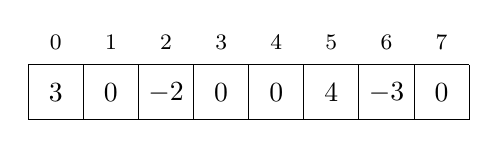
\begin{tikzpicture}[scale=0.7]
\draw (0,0) grid (8,1);

\node at (0.5,0.5) {$3$};
\node at (1.5,0.5) {$0$};
\node at (2.5,0.5) {$-2$};
\node at (3.5,0.5) {$0$};
\node at (4.5,0.5) {$0$};
\node at (5.5,0.5) {$4$};
\node at (6.5,0.5) {$-3$};
\node at (7.5,0.5) {$0$};


\footnotesize
\node at (0.5,1.4) {$0$};
\node at (1.5,1.4) {$1$};
\node at (2.5,1.4) {$2$};
\node at (3.5,1.4) {$3$};
\node at (4.5,1.4) {$4$};
\node at (5.5,1.4) {$5$};
\node at (6.5,1.4) {$6$};
\node at (7.5,1.4) {$7$};
\end{tikzpicture}
\end{center}

Por ejemplo, el valor 2 en la posición 6 del array original
corresponde a la suma $3-2+4-3=2$ en el array de diferencias.

La ventaja del array de diferencias es
que podemos actualizar un rango
en el array original cambiando solo
dos elementos en el array de diferencias.
Por ejemplo, si queremos
aumentar los valores del array original
entre las posiciones 1 y 4 en 5,
basta con aumentar el valor del
array de diferencias en la posición 1 en 5
y disminuir el valor en la posición 5 en 5.
El resultado es el siguiente:

\begin{center}
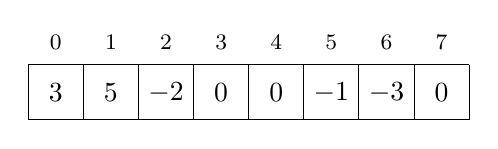
\begin{tikzpicture}[scale=0.7]
\draw (0,0) grid (8,1);

\node at (0.5,0.5) {$3$};
\node at (1.5,0.5) {$5$};
\node at (2.5,0.5) {$-2$};
\node at (3.5,0.5) {$0$};
\node at (4.5,0.5) {$0$};
\node at (5.5,0.5) {$-1$};
\node at (6.5,0.5) {$-3$};
\node at (7.5,0.5) {$0$};

\footnotesize
\node at (0.5,1.4) {$0$};
\node at (1.5,1.4) {$1$};
\node at (2.5,1.4) {$2$};
\node at (3.5,1.4) {$3$};
\node at (4.5,1.4) {$4$};
\node at (5.5,1.4) {$5$};
\node at (6.5,1.4) {$6$};
\node at (7.5,1.4) {$7$};
\end{tikzpicture}
\end{center}

Más generalmente, para aumentar los valores
en el rango $[a,b]$ en $x$,
aumentamos el valor en la posición $a$ en $x$
y disminuimos el valor en la posición $b+1$ en $x$.
Por lo tanto, solo es necesario actualizar valores únicos
y procesar consultas de suma,
por lo que podemos usar un árbol indexado binario o un árbol de segmentos.

Un problema más difícil es soportar ambos
consultas de rango y actualizaciones de rango.
En el Capítulo 28 veremos que incluso esto es posible. 
